\originalchapter{作业 2}
MIT 18.330, Spring 2012. 原件: Homework 2, Due March 1. 以下解答均为 AI 编写, 非官方答案. 原件说明: 求数值时可用任何方法, 包括解析或符号方法, 但须说明取得答案的方法.

\begin{exercise}\label{ps2-q1}
(原题 1, 1 分) 设 $\alpha,\beta$ 为实数. 若 $h\to0$ 时 $f(h)=O(h^\alpha)$, 证明 $h^\beta f(h)=O(h^{\alpha+\beta})$.
\end{exercise}
\begin{solution}
对实数次幂按数值分析惯例取 $h\to0^+$. 存在 $C,h_0>0$, 使 $0<h<h_0$ 时 $|f(h)|\le Ch^\alpha$. 乘以正数 $h^\beta$ 得 $|h^\beta f(h)|\le Ch^{\alpha+\beta}$. 若用双侧极限, 应将各幂明确写作 $|h|$ 的幂.
\end{solution}

\begin{exercise}\label{ps2-q2}
(原题 2, 2 分) 考虑中点法
$\int_0^1 f(x)\dd x\simeq h\sum_{j=0}^{N-1}f((j+1/2)h)$, $h=1/N$.
画图解释“中点”的含义. 该法的精度阶是多少? 证明你的答案.
\end{exercise}
\begin{solution}
每小区间用宽 $h$、高为中点函数值的矩形近似曲线下方面积. 下图为 $f(x)=1+x^2$, $N=4$ 的示意.
\begin{center}
\begin{tikzpicture}[x=6cm,y=1.4cm]
\draw[->] (0,0)--(1.08,0) node[right] {$x$};
\draw[->] (0,0)--(0,2.3) node[above] {$f$};
\foreach \j in {0,1,2,3}{
\pgfmathsetmacro{\l}{\j/4}\pgfmathsetmacro{\r}{(\j+1)/4}
\pgfmathsetmacro{\m}{(\j+.5)/4}\pgfmathsetmacro{\v}{1+\m*\m}
\draw[structurecolor] (\l,0)--(\l,\v)--(\r,\v)--(\r,0);
\fill (\m,\v) circle(1pt);}
\draw[thick,domain=0:1,samples=80] plot(\x,{1+\x*\x});
\node[below] at (1,0) {$1$};
\end{tikzpicture}
\end{center}
假设 $f\in C^2[0,1]$, 令中点 $m_j=(j+1/2)h$. Taylor 展开的一次项关于中点对称积分后消失, 余项绝对值不超过 $\|f''\|_\infty(x-m_j)^2/2$, 因而每格误差不超过 $\|f''\|_\infty h^3/24$. 求和 $N=1/h$ 格得总误差 $O(h^2)$. 对 $f=x^2$ 总误差恰为 $h^2/12$, 故一般精度确为二阶.
\end{solution}

\begin{exercise}\label{ps2-q3}
(原题 3, 3 分) 在 $[-1,2]$ 上考虑 $f(x)=x/(1+x^4)$. 写脚本实现一阶矩形法与二阶梯形法. 此时可学习 MATLAB 的向量运算和 \texttt{sum} 命令.
\begin{enumerate}[label=\textbullet]
\item 区间从 $[0,1]$ 换成 $[-1,2]$ 后求积公式怎样写? 特别说明 $h$ 与 $N$ 的关系以及网格点 $x_j$ 的选取.
\item 求 $\int_{-1}^2 f(x)\dd x$, 精确到小数点后 10 位.
\item 画两种方法的绝对截断误差关于 $h$ 的双对数图; $h$ 的范围应跨越数个数量级. 解释如何从图中读出收敛阶.
\end{enumerate}
\end{exercise}
\begin{solution}
取 $h=3/N$, $x_j=-1+jh$, $0\le j\le N$. 左端矩形与复合梯形分别为
\[
R_h=h\sum_{j=0}^{N-1}f(x_j),\qquad
T_h=h\left[\frac{f(x_0)+f(x_N)}2+\sum_{j=1}^{N-1}f(x_j)\right].
\]
原函数为 $\frac12\arctan(x^2)$, 所以积分为
$\frac12(\arctan4-\arctan1)=0.2702097501$.
实际使用 $N=2^5,\ldots,2^{15}$; 双对数图中 $E\sim Ch^p$ 表现为斜率 $p$ 的直线. 最细五组数据拟合斜率约为 $1.000$ 与 $2.000$; 避开舍入误差主导区间. 同一脚本保存全部误差数据.
\begin{center}
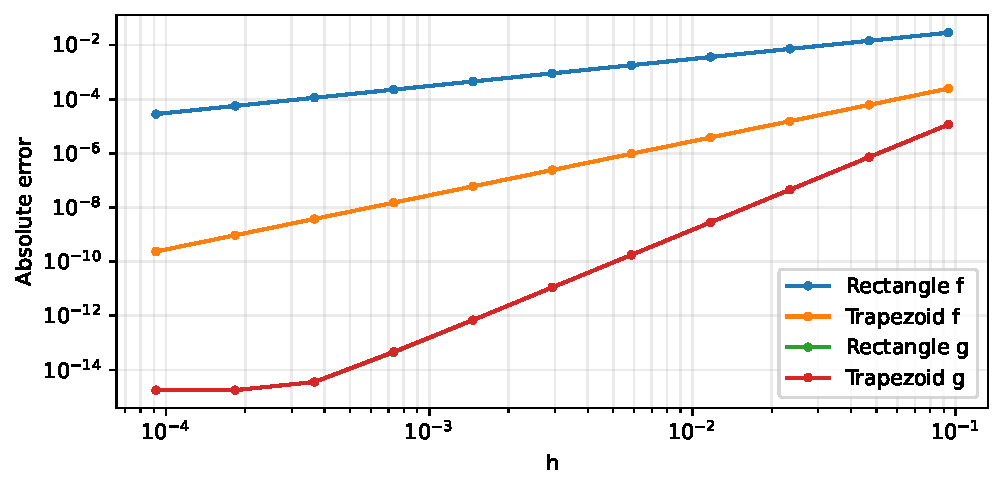
\includegraphics[width=.9\linewidth]{figures/assessments/ps2_quadrature.pdf}
\end{center}
上图的另外两条曲线对应下一题的 $g$. 数值证据与 Taylor/Euler--Maclaurin 给出的理论阶一致.
\end{solution}

\begin{exercise}\label{ps2-q4}
(原题 4, 1 分) 将第 3 题的函数改为 $g(x)=(x+1)^3(x-2)^2$, 在同一区间 $[-1,2]$ 重画收敛图. 两种方法现在各有几阶精度? (附加 1 分: 解释观察到的现象.)
\end{exercise}
\begin{solution}
实际两条误差曲线重合, 都为四阶. 由于 $g(-1)=g(2)=0$, $R_h=T_h$; 且 $g'(-1)=g'(2)=0$, 梯形的二阶主项消失. 用 Euler--Maclaurin 对五次多项式的精确有限展开,
\[
T_h-\int_{-1}^2g(x)\dd x
=\frac{h^2}{12}[g'(2)-g'(-1)]
-\frac{h^4}{720}[g'''(2)-g'''(-1)]= -\frac{3}{20}h^4.
\]
这里 $g'''(2)-g'''(-1)=108$; 后续项的端点导数差为零. 用 $t=x+1$ 积分 $t^3(t-3)^2$ 得真值 $3^6/60=12.15$. 拟合四阶曲线时须避开误差已接近机器精度的最细网格; 理论公式可直接核对每一行数值.
\end{solution}

\begin{exercise}\label{ps2-q5}
(原题 5, 3 分) 仍取 $f(x)=x/(1+x^4)$, 编写脚本实现一阶前向差分与二阶中心差分. 在间距 $h$ 的细网格上计算每个点的导数, 排除两个端点; 可沿用前题的网格约定.
\begin{enumerate}[label=\textbullet]
\item 求 $f'(1)$, 精确到小数点后 10 位.
\item 画截断误差关于 $h$ 的双对数图. 误差取所有内点上数值导数与精确导数之差的绝对值的最大值; 高精度数值导数也可代替精确值. 解释如何从图中看出收敛阶.
\end{enumerate}
\end{exercise}
\begin{solution}
解析微分得 $f'(x)=(1-3x^4)/(1+x^4)^2$, 故 $f'(1)=-0.5000000000$. 内点使用
$D_+f_j=(f_{j+1}-f_j)/h$,
$D_0f_j=(f_{j+1}-f_{j-1})/(2h)$, 与解析导数逐点比较.
一致 Taylor 估计分别给出 $O(h)$ 和 $O(h^2)$; 实际最大范数误差曲线的斜率约为 $1.000$ 和 $2.000$.
\begin{center}
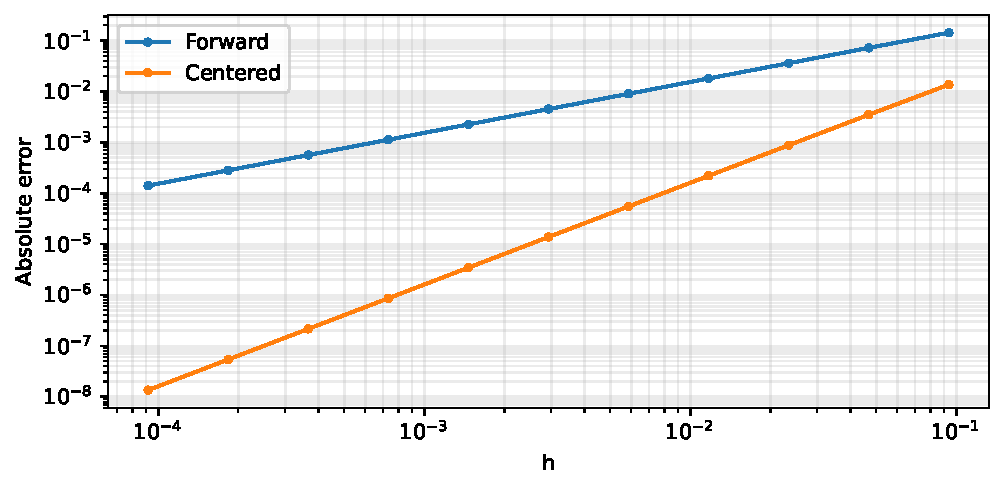
\includegraphics[width=.86\linewidth]{figures/assessments/ps2_differences.pdf}
\end{center}
源码以数组 \texttt{y[2:]-y[1:-1]} 和 \texttt{y[2:]-y[:-2]} 计算, 确保两种误差都只比较相同的内点.
\end{solution}
